\documentclass{article}

\usepackage{tabularx}
\usepackage{booktabs}
\usepackage[explicit]{titlesec}
\usepackage{fullpage}
\usepackage{titling}
\usepackage{hyperref}
\usepackage{graphicx}
\usepackage{float}

\setlength{\droptitle}{-14ex}  

\titleformat{\section}
  {\normalfont\large\bfseries}{\thesection}{1em}{{#1}}

\titleformat{\subsection}
  {\normalfont\bfseries}{\thesection}{1em}{{#1}}

\title{CAS 741: Problem Statement\\[10pt]\Large Dynamical Systems: Multi-Pendulum }

\author{Karol Serkis\\\texttt{serkiskj@mcmaster.ca}}

\date{}

\usepackage{color}

%\newif\ifcomments\commentstrue

%\ifcomments
%\newcommand{\authornote}[3]{\textcolor{#1}{[#3 ---#2]}}
%\newcommand{\todo}[1]{\textcolor{red}{[TODO: #1]}}
%\else
%\newcommand{\authornote}[3]{}
%\newcommand{\todo}[1]{}
%\fi

%\newcommand{\wss}[1]{\authornote{blue}{SS}{#1}}
%\newcommand{\spc}[1]{\authornote{magenta}{SP}{#1}}

%% Comments

\usepackage{color}

\newif\ifcomments\commentsfalse

\ifcomments
\newcommand{\authornote}[3]{\textcolor{#1}{[#3 ---#2]}}
\newcommand{\todo}[1]{\textcolor{red}{[TODO: #1]}}
\else
\newcommand{\authornote}[3]{}
\newcommand{\todo}[1]{}
\fi

\newcommand{\wss}[1]{\authornote{blue}{SS}{#1}}
\newcommand{\spc}[1]{\authornote{magenta}{SP}{#1}}

\begin{document}

%\pagenumbering{gobble}

\maketitle

\begin{table}[hp]
\caption{Revision History} \label{TblRevisionHistory}
\begin{tabularx}{\textwidth}{llX}
\toprule
\textbf{Date} & \textbf{Developer(s)} & \textbf{Change}\\
\midrule
September 17, 2018 & Karol Serkis & First revision of document\\
September 14, 2018 & Karol Serkis & Problem Idea proposed \& discussed with Dr.
Spencer Smith \\
\bottomrule
\end{tabularx}
\end{table}

\wss{Why reproduce the contents of the Comments.tex file?  It was written
  separately so that it can easily be included in every document.}

\section*{Problem}

\wss{Please keep the lines of tex to a fixed width (say 80 characters) so that
  it is easier to do diffs between commits.  Your tex editor should have a
  facility for doing this.}

A simple gravity pendulum has very easy to system to model and consists of a
weight suspended from a pivot and the weight is given enough space to swing
freely. To simplify the model we assume no air resistance with a frictionless
pivot [1]. The model and calculations for the simple gravity pendulum are well
defined and only require ordinary differential equation (ODE) solvers as well as 
Lagrangian and/or Hamiltonian mechanics equations.
[2]. \wss{Are you also assuming a small angle?  Usually that is an assumption
  made so that sin(theta) is approximately equal to theta.}
\begin{figure}[H]
	\centering
	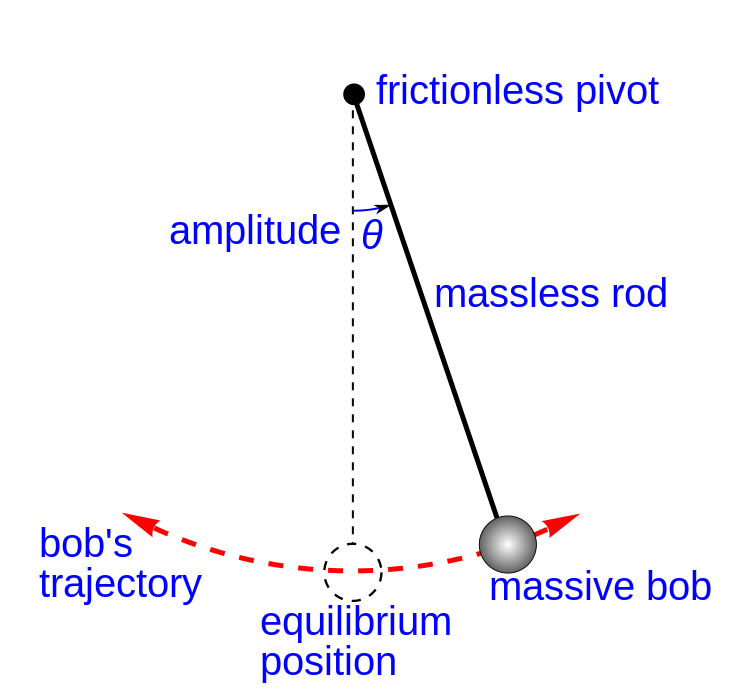
\includegraphics[width=250px]{simple-pend.png}
\caption{A simple gravity pendulum where the model assumes no friction or air
resistance [1]}
	\label{fig:maxresdefault}
\end{figure}

However, once you attach a pendulum to the bottom of another pendulum in the
case of a double pendulum you have a new system that is dynamic and chaotic and
requires a set of coupled ordinary differential equation solvers [3]. Once you
introduce multiple pendula the system becomes chaotic and interesting to model
and simulate.

\begin{figure}[H]
	\centering
	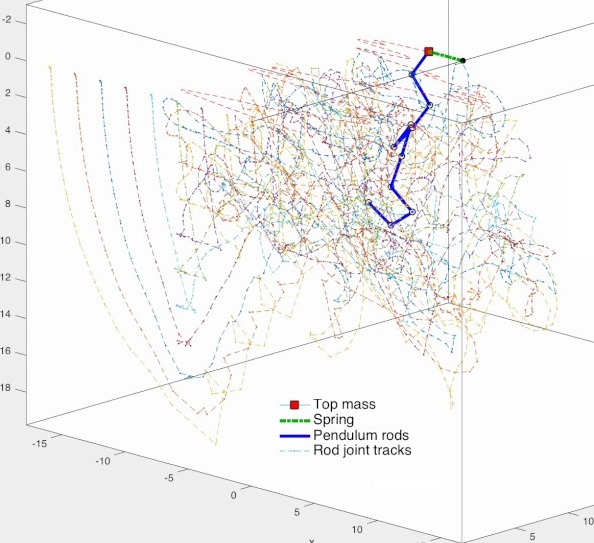
\includegraphics[width=220px]{multi-pend.jpg}
\caption{An example of dynamical and chaoitc system with
Spring-Mass-Multi-Pendulum [5]}
	\label{fig:maxresdefault}
\end{figure}

\section*{Proposed Solution}
A proposed software solution will produce a simulation of a multi-pendulum
system. Inspiration for this problem came from Dr. Ned Nedialkov's Multi-body
Lagrangian Simulations using DAETS (Differential-Algebraic Equations by Taylor
Series). DAETS is a C++ package for solving initial value problems for DAE
systems [4].

\begin{figure}[H]
	\centering
	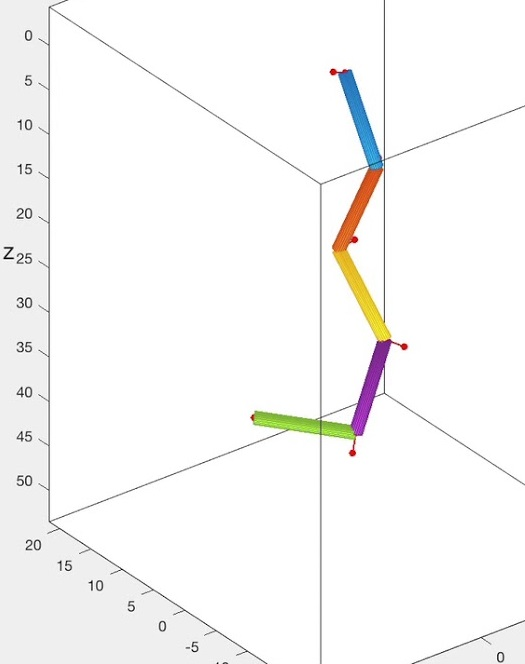
\includegraphics[width=150px]{3pend.jpg}
	\caption{Simulation of Multi-Pendulum system using DAETS [5]}
	\label{fig:maxresdefault}
\end{figure}

The proposed software is to develop a multi-platform equivalent solution that
only focuses on multi-pendulum simulations and tracking the chaotic motion of
the system. It will allow users to generate diagrams and plot trajectories over
time using two different ODE/DAE initial value problem solvers [4]. 
Multiple solvers can be compared for performance and accuracy.
 \wss{Rather than say ``If time allows,''  you can just make this part
  of the original project.  If it has to be dropped out, we can ``fake'' this
  document later, or simply modify your requirements document.}

\section*{Context}
\subsection*{Environment}
The simulation software will be created with multi-platform support in mind and
be compatible with Windows 10, Mac OS, Linux, etc. In order to achieve this,
Python and/or MATLAB will be used for development of the software.

\subsection*{Stakeholders}
Specific stakeholders include:
\begin{itemize}
\item Karol Serkis
\item Dr. Spencer Smith
\item Dr. Ned Nedialov
\item Students of CAS 741 
\item Individuals studying or working in fields related to physics
\end{itemize}

\subsection*{References}
\begin{itemize}
\item{[1]} Pendulum \\\url{https://en.wikipedia.org/wiki/Pendulum}
\item{[2]} Pendulum (mathematics)
\\\url{https://en.wikipedia.org/wiki/Pendulum_(mathematics)}
\item{[3]} Double Pendulum \\\url{https://en.wikipedia.org/wiki/Double_pendulum}
\item{[4]} Differential-Algebraic Equations by Taylor Series
\\\url{http://www.cas.mcmaster.ca/~nedialk/daets/}
\item{[5]} Multi-body Lagrangian Simulations
\\\url{https://www.youtube.com/channel/UCCuLchOx0W0yoNE9KOCYlVQ}
\end{itemize}

\end{document}